\documentclass[10pt,twocolumn,letterpaper]{article}

\usepackage{cvpr}
\usepackage{times}
\usepackage{epsfig}
\usepackage{graphicx}
\usepackage{amsmath}
\usepackage{amssymb}
\usepackage{listings}
\usepackage{algorithm}
\usepackage[noend]{algpseudocode}
\usepackage{fancyvrb}
\usepackage{xcolor}
\usepackage{tabularx}
\usepackage[T1]{fontenc}
\makeatletter
\@namedef{ver@everyshi.sty}{}
\makeatother
\usepackage{pgfplots} 

\usepackage{url}


\cvprfinalcopy % *** Uncomment this line for the final submission

\def\cvprPaperID{****} % *** Enter the CVPR Paper ID here
\def\httilde{\mbox{\tt\raisebox{-.5ex}{\symbol{126}}}}

\makeatletter
\def\BState{\State\hskip-\ALG@thistlm}
\makeatother

% Needed to show code snippets...
\DefineVerbatimEnvironment{Highlighting}{Verbatim}{commandchars=\\\{\}}
\newenvironment{Shaded}{}{}
\newcommand{\StringTok}[1]{\textcolor[rgb]{0.25,0.44,0.63}{#1}}
\newcommand{\AttributeTok}[1]{\textcolor[rgb]{0.49,0.56,0.16}{#1}}
\newcommand{\ExtensionTok}[1]{#1}
\newcommand{\NormalTok}[1]{#1}

% Algorithm Custom Indent
\makeatletter
\let\OldStatex\Statex
\renewcommand{\Statex}[1][3]{%
  \setlength\@tempdima{\algorithmicindent}%
  \OldStatex\hskip\dimexpr#1\@tempdima\relax}
\makeatother

\makeatletter
\algrenewcommand\ALG@beginalgorithmic{\scriptsize}
\makeatother
%

\lstdefinestyle{CSnippetStyle}{
  language=C,
  numbers=left,
  stepnumber=1,
  numbersep=10pt,
  tabsize=2,
  breaklines=true,
  postbreak=\mbox{\textcolor{red}{$\hookrightarrow$}\space},
  showspaces=false,
  numbersep=5pt,
  showstringspaces=false,
  captionpos=b,
  % Colors and Font
  basicstyle=\footnotesize\ttfamily,
  keywordstyle=\bfseries\color{green!40!black},
  commentstyle=\itshape\color{purple!40!black},
  identifierstyle=\color{blue},
  stringstyle=\color{orange},
}

\graphicspath{ {./images/} }



% Pages are numbered in submission mode, and unnumbered in camera-ready
\ifcvprfinal\pagestyle{empty}\fi
\begin{document}

%%%%%%%%% TITLE
\title{DES Password Decrypter}

\author{Adriano Di Dio\\
E-mail address\\
{\tt\small adriano.didio@stud.unifi.it}
}

\maketitle
\thispagestyle{empty}

%%%%%%%%% ABSTRACT
\begin{abstract}
Purpose of this paper is to describe how to decrypt a DES hashed password using brute-force.\newline
In particular, it will be shown how to implement the main algorithm in C and how it can be sped up using multiple threads through the 
pthreads library.
\end{abstract}

%%%%%%%%% BODY TEXT
\noindent\large\textbf{Future Distribution Permission}\\
\indent The author(s) of this report give permission for this document to be distributed to Unifi-affiliated students taking future courses.

\section{Introduction}
Data Encryption Standard (DES) is a symmetric-key algorithm used for the encryption of data.\\
DES passwords can be generated using a library available for the C programming language called `libcrypt' that exposes two versions of 
the same function named: crypt and crypt\_r.\\
The first one is the standard and will be used in the sequential version, while the latter is the reentrant version of the same function 
which is required when dealing with multiple threads due to the possibility of the scheduler to interrupt any thread at any time, 
causing the library to not complete the encryption operation and returning invalid data.\\
Differences about the two function will be given in the chapters related to the sequential and parallel version.\\
In particular in chapter 2 a brief explanation of the algorithm is given,then in chapter 3 and 4 the sequential and parallel version is 
described, and finally, in the last chapter, the performance will be evaluated by showing the differences between the two approaches.\\ 

\vspace{3cm}

%-------------------------------------------------------------------------
\section{Algorithm}

Every password created using the crypt function has the following format:\\
\begin{Shaded}
\begin{Highlighting}[]
\ExtensionTok{salt+hash}
\end{Highlighting}
\end{Shaded}
the salt is used as a countermeasure to specific attacks such as the Rainbow Table method where an attacker could generate a list of 
hashed password that can be combined to find the correspondent plain-text one, in fact, by adding a random salt,that should be removed 
from the final password, these kind of attack could be mitigated due to the necessity of knowing which salt has been applied.\\
In our case, the salt is always known since it is given by the user itself when running the decrypt program.\\
The brute-force attack, is a process where the attacker tries all the possible available combination of a specific charset.\\
As an example, this is the default charset that will be used in the implementation:\\

\begin{figure}[H]\label{default-charset}
\begin{footnotesize}
abcdefghilmnopqrstuvzABCDEFGHILMNOPQRSTUVZ0123456789./
\end{footnotesize}
\caption{Default Charset}
\end{figure}

the algorithm is quite simple and the main objective is to find all the possible combination of the letters available in the charset and
run, for each combination, the crypt function to test if the hashed password matches the one that was given from the user.\\
Below, a pseudo-code implementation, to describe the algorithm:\\
\begin{algorithm}
\caption{Password Decrypter\newline
Takes 4 parameters:Password,Salt,Charset,Password Length}\label{euclid}
\begin{algorithmic}[1]
\Procedure{GuessPassword}{Password,Salt,Charset,Length}
	
    \State Let ${CurrentCombination}$ a new list of length $\gets {Length}$
    \State Let ${Position}$ a new list of length $\gets {Length}$
	\For{\texttt{$i \gets 0$ to $Length$}}
    	\State {$Combination[i]$ $\gets$ {$Charset[0]$}}
    	\State {$Position[i]$ $\gets$ {$Charset[0]$}}
	\EndFor
	
    \While{True}
        \Statex \Call{crypt}{$Combination$,$Salt$} $\gets {Hash}$
        
        \If {$Hash == Password$}
            \State \Return $Combination$
        \EndIf
        \State $Place$ $\gets {Length - 1}$
        \While{$Place >= 0$}
            \State $Position[Place]$ $\gets {Position[Place] + 1}$
			\State $Len$ $\gets {len(Charset)}$
            \If {$Position[Place] == Len$}
            	\State $Position[Place]$ $\gets {0}$
                \State $Combination[Place]$ $\gets {Charset[0]}$
                \State $Place$ $\gets {Place - 1}$
            \Else
            	\State $Letter$ $\gets {Charset[Place]}$
            	\State $Combination[Place]$ $\gets {Letter}$
            	\State \textbf{break}
            \EndIf
        \EndWhile
        \If {$Place < 0 $}
	        \State \textbf{break}
        \EndIf
    \EndWhile
   	\State \Return $""$
\EndProcedure
\\
\Procedure{Decrypt}{MaxLength}
	\For{\texttt{$i \gets 1$ to $MaxLength$}}
		\State \Call{GuessPassword}{$Password,MaxLength$} $\gets {Password}$
            \If {$Password \neq ""$}
				\State \Return $Password$
			\EndIf
	\EndFor
	\State \Return $""$
\EndProcedure
\end{algorithmic}
\end{algorithm}


As we can see from the pseudo-code the algorithm is quite simple, and it works like a counter that produces all the available 
combination from the given charset.\\
In particular the entry function is called decrypt, which calls the GuessByLength function in a loop that goes from 1 to the maximum 
allowed password length,which calculates all the possible combinations.\\
Inside the GuessByLength function we have the main algorithm that generates the possible combinations.\\
In the first part, we initialize two arrays, Position and Combination, that are used respectively as the Counter and the corresponding
combination based on the counter values.\\
Then the loop is started and the first combination is checked by calling the crypt function that produces the hash for the current 
combination and salt, and returns the hash value as a string that can be compared to the encrypted password, if it matches the function
returns the plain-text password otherwise it creates a new combination by Starting from the maximum length of the password and adding to
the counter the current position relative to the charset.\\
When the counter has reached the last letter of the charset, it wraps around, and start a new count on the other element of the array.\\
If all the values have been tried then the main loop is stopped and the function returns an empty string otherwise it will keep 
iterating until one of the previous condition is met.\\
When the function `GuessByLength' returns, the decrypt function that called it, checks if the returned password is not empty and it will 
stop the iteration and returns the result to the user,otherwise it will keep iterating until the max length is reached.\\

\section{Implementation}
\subsection{Tools}
A tool has been written in C to generate a DES password, using the crypt function, and requires only two parameters:the plain-text 
password and the salt.\\
It returns the encrypted password that can be later used in the decrypt application to test it out.\\
E.G\\
\begin{Shaded}
\begin{Highlighting}[]
\NormalTok{\$ }\ExtensionTok{./Crypt foo aa}
\end{Highlighting}
\end{Shaded}
Sample Output:\\
\begin{Shaded}
\begin{Highlighting}[]
\NormalTok{\$ }\ExtensionTok{Crypted Password for foo is \ldots}
\end{Highlighting}
\end{Shaded}

\subsection{Main Program}
The algorithm, seen in the pseudo-code,is implemented in both the sequential version and in the parallel one in C but the implementation 
is slightly different in the parallel one to optimize thread usages.\\
\subsubsection{Sequential Version}
The sequential version is made using two functions as seen in the pseudocode, one for iterating over the maximum allowed length while 
the other to create the possible combinations.\\
The following structure have been declared to initialize a decrypt session:
\begin{lstinputlisting}[language=C,style=CSnippetStyle,caption=Data Structure Definition ]{
	"codes/Sequential/Decrypt.h"}
\end{lstinputlisting}

this structure is initialized in the main function as it can be seen below:
\begin{lstinputlisting}[language=C,style=CSnippetStyle,caption=DecypherSettingsInit Function,firstline=93,lastline=113 ]{
	"codes/Sequential/Decrypt.c"}
\end{lstinputlisting}
and contains all the data needed to implement the algorithm, the Decrypted Password field will be populated once the algorithm has 
finished and a password was found,the charset can be set from the command line or it can use the default one which is:
\begin{lstinputlisting}[language=C,style=CSnippetStyle,caption=Default Charset,firstline=3,lastline=3]{
	"codes/Sequential/Decrypt.c"}
\end{lstinputlisting}
After initialization the decrypt function is called, passing the previous initialized data structure (DecypherSettings), and the 
algorithm starts:
\begin{lstinputlisting}[language=C,style=CSnippetStyle,caption=Decrypt Function,firstline=71,lastline=91]{
	"codes/Sequential/Decrypt.c"}
\end{lstinputlisting}
This function, as seen in the pseudo-code, calls `GuessPasswordByLength' with an increasing MaxLength until either the password is found
or the length has reached the maximum value.\\
The function can be seen in below snippet:\\
\begin{lstinputlisting}[language=C,style=CSnippetStyle,caption=GuessPasswordByLength Function,firstline=27,lastline=69]{
	"codes/Sequential/Decrypt.c"}
\end{lstinputlisting}
where the function is implemented, in the same way as seen in the pseudo-code, it will generate all possible combination given the 
maximum length and for each combination it will call the `ComparePassword function':
\begin{lstinputlisting}[language=C,style=CSnippetStyle,caption=ComparePassword Function,firstline=20,lastline=25]{
	"codes/Sequential/Decrypt.c"}
\end{lstinputlisting}
that, as it can be seen by the snippet above, calculates an hash with the same salt as the one the user passed to the program and if
the two hash matches then the plain-text password is returned based on the current combination used to generate it.\\
When this function returns 1 then the password has been found and the loop in the Decrypt function is interrupted in order to print out 
the plain-text password along with the execution time in ms.\\
If the password is not found and the loop has reached his maximum value then a message will inform the user that the password could not
be decrypted.\\
\subsection{Usage}
To use the application, user needs to specify only the encrypted password and the maximum length:\\
\begin{Shaded}
\begin{Highlighting}[]
\NormalTok{\$ }\ExtensionTok{./PasswordDecrypterSP asgCdZs 8}
\end{Highlighting}
\end{Shaded}
If the user want to change the charset, they can be modified by using the following command-line option:\\
\begin{Shaded}
\begin{Highlighting}[]
\NormalTok{\$ }\ExtensionTok{/PasswordDecrypterMP --Charset abcd}
\end{Highlighting}
\end{Shaded}
By default the charset is the one seen in figure \ref{default-charset}
\subsection{Parallel Version}
As we can see from the pseudo-code, the generation of all the possible combination can be done in parallel by distributing the available
combination to multiple threads that can check if the password match in parallel without having to wait.\\
The following data structures have been declared to hold the status of the decrypter between multiple threads:\\
\begin{lstinputlisting}[language=C,style=CSnippetStyle,caption=Parallel Data Structure,firstline=1,lastline=33]{
	"codes/Parallel/Decrypt.c"}
\end{lstinputlisting}
in the DecypherSettings structure we have the same data as the one seen in the sequential version that holds the configuration for the 
decryption session that we need to run, and it is initialized in the same way:
\begin{lstinputlisting}[language=C,style=CSnippetStyle,caption=Decrypter Session Data Structure 
	Initialization,firstline=212,lastline=223]{"codes/Parallel/Decrypt.c"}
\end{lstinputlisting}
then, the thread structure is initialized by defining the starting conditions:\\
\begin{lstinputlisting}[language=C,style=CSnippetStyle,caption=Parallel Data Structure 
			Initialization,firstline=225,lastline=236]{"codes/Parallel/Decrypt.c"}
\end{lstinputlisting}
As we can see from the above snippet the program uses one mutex and one condition to handle thread synchronization, and a pool of four
workers threads to generate the available combinations.\\
Note that the number of workers can be set from command-line.\\
The actual thread are then started:\\
\begin{lstinputlisting}[language=C,style=CSnippetStyle,caption=Thread Launch,firstline=238,lastline=241]{"codes/Parallel/Decrypt.c"}
\end{lstinputlisting}
there are two types of thread, the first one is the Master which handles thread synchronization when an exit event occur while the 
others are the workers thread which do the actual required job.\\
The master thread is only one and uses the following function:\\
\begin{lstinputlisting}[language=C,style=CSnippetStyle,caption=Master Thread,firstline=170,lastline=196]{"codes/Parallel/Decrypt.c"}
\end{lstinputlisting}
as we can see from the snippet, the master thread will wait until an exit condition occurs.\\
An exit condition happens when either one worker finds the password or when a worker has reached the maximum allowed combination given
the maximum length, when one of these events occurs the worker broadcast a signal that wakes up the master thread that will look to the
shared data structure to see what exit code the worker has put into the variable JobStatus.\\
If the JobStatus is equals to `decrypter\_job\_Status\_found' then the master thread will cancel all the running worker threads using 
the function `pthread\_cancel' and waits for their termination using the `pthread\_join' function otherwise, if the JobStatus is 
equals to `decrypter\_job\_status\_reached\_max\_combination' then it will wait for normal termination of all the worker threads by 
calling the `pthread\_join'.\\
When all the threads have joined, the master will exit, terminating itself.\\
The workers uses a different function which is called `DoWork`.\\
It is important to note that in order to avoid any overhead when dealing with trivial passwords, the workers thread must be initialized
as follows:\\
\begin{lstinputlisting}[language=C,style=CSnippetStyle,caption=Worker Thread Initialization,firstline=116,lastline=117]
		{"codes/Parallel/Decrypt.c"}
\end{lstinputlisting}
this ensures that the threads could be cancelled at any time without having to wait for a specific cancellation point.\\
Then every worker thread must initialize the data structure required by the reentrant crypt function as shown below:\\
\begin{lstinputlisting}[language=C,style=CSnippetStyle,caption=Crypt Function Initialization,firstline=110,lastline=112]
		{"codes/Parallel/Decrypt.c"}
\end{lstinputlisting}
if the initialized value is not zero or is not set then the crypt function will not work properly.\\
After initialization the main worker thread code is executed as an infinite while loop, on every iteration the worker checks if there 
are any available jobs by calling the function `PoolGetAvailableJob':\\
\begin{lstinputlisting}[language=C,style=CSnippetStyle,caption=PoolGetAvailableJob Function,firstline=120,lastline=120]
		{"codes/Parallel/Decrypt.c"}
\end{lstinputlisting}
this function checks the current status of the decryption session and advances the counter till the maximum allowed length is reached.\\
Since the data structure is shared a mutex is used to avoid any data race as seen below:\\
\begin{lstinputlisting}[language=C,style=CSnippetStyle,caption=PoolGetAvailableJob Function,firstline=57,lastline=87]
		{"codes/Parallel/Decrypt.c"}
\end{lstinputlisting}
this function generates a new job that the worker can do by giving a range of combination that it can generates, the range size depends
from the `CharsetIncrement' variable that holds the size of each chunk.\\
When the maximum length is reached, it will return NULL and the worker thread will broadcast the exit condition to the master
thread:\\
\begin{lstinputlisting}[language=C,style=CSnippetStyle,caption=Worker Exit,firstline=121,lastline=124]
		{"codes/Parallel/Decrypt.c"}
\end{lstinputlisting}
otherwise, the worker will generate all the combination in the given range:
\begin{lstinputlisting}[language=C,style=CSnippetStyle,caption=Worker Combination Generator,firstline=139,lastline=163]
		{"codes/Parallel/Decrypt.c"}
\end{lstinputlisting}
As we can see from above there are two utilities function:`WorkerHasReachedMaxCombination' and `ComparePassword'.\\
`WorkerHasReachedMaxCombination' simply checks if the worker has completed his job by comparing the current counter status with the
target one:\\
\begin{lstinputlisting}[language=C,style=CSnippetStyle,caption=WorkerHasReachedMaxCombination Function,firstline=42,lastline=55]
		{"codes/Parallel/Decrypt.c"}
\end{lstinputlisting}
while `ComparePassword' calls the crypt\_r function, along with his data structure, and check if the hash of the current 
combination matches the password:\\
\begin{lstinputlisting}[language=C,style=CSnippetStyle,caption=Compare Password Function,firstline=35,lastline=40]
		{"codes/Parallel/Decrypt.c"}
\end{lstinputlisting}
if it does then the worker thread will save it to the shared data structure and will wake up the master in order to terminates all the
running threads.\\
The exit function is shown below:\\
\begin{lstinputlisting}[language=C,style=CSnippetStyle,caption=Worker Exit Function,firstline=88,lastline=98]
		{"codes/Parallel/Decrypt.c"}
\end{lstinputlisting}
Finally the program will exit when the master thread exit which is detected using the `pthread\_join' statement.\\
The parallel implementation has been profiled using Intel's Vtune-profiler which showed no data races and full CPU cores usage,altough
as we can see from the image it warned about some issues about being memory bound.\\
\subsection{Usage}
To use the application, user needs to specify only the encrypted password and the maximum length:\\
\begin{Shaded}
\begin{Highlighting}[]
\NormalTok{\$ }\ExtensionTok{./PasswordDecrypterMP asgCdZs 8}
\end{Highlighting}
\end{Shaded}
If the user want to increase the number of workers threads or change the charset, they can be modified by using two command-line 
options:\\
\begin{Shaded}
\begin{Highlighting}[]
\NormalTok{\$ }/PasswordDecrypterMP \\
--NumThreads 8 --Charset abcd
\end{Highlighting}
\end{Shaded}
By default the number of threads is four and the charset is the one seen in figure \ref{default-charset}

\begin{figure}[H]
\centering
\includegraphics[width=0.5\textwidth]{vtune_profiler}
\caption{Intel's VTune-Profiler}
\end{figure}
These issues were actually related to the libCrypto, which the program uses to test if the password matches, and cannot be directly 
fixed.
\section{Metrics}
\subsection{Run-Time Comparison}
In order to see what advantages the parallel implementation has brought we need to measure the execution time of both implementations by
using the same passwords.\\
The processor, used to collect the data, is an `Intel(R) Core(TM) i5-4200M CPU' that has two cores and 4 hardware threads.\\
The execution time is measured using the same function:\\
\begin{lstinputlisting}[language=C,style=CSnippetStyle,caption=Time Function,firstline=1,lastline=13]
		{"codes/Metrics.c"}
\end{lstinputlisting}
that measures the elapsed time in milliseconds.\\
Under the hood it uses the function `gettimeofday()' that returns the Wall Clock and the results are available in the following table:
\\
\begin{table}[H]
 \begin{tabularx}{\columnwidth}{X|X|X|X|}
\textbf{Password} & \textbf{SP Time} & \textbf{MP Time} &  \textbf{SpeedUp} \\
foo & 60 ms & 21 ms & 2.85 \\
fooB & 3005 ms & 1157 ms & 2.59 \\
foobB & 164411 ms & 64443 ms & 2.55 \\
foobbB & 171,612 m & 72.84 m & 2.35 \\
\end{tabularx}
\caption{Execution Times}
\end{table}
\subsection{Parallel Run-time vs Number Of Threads}\label{run-time-vs-num-threads}

\begin{figure}[H]
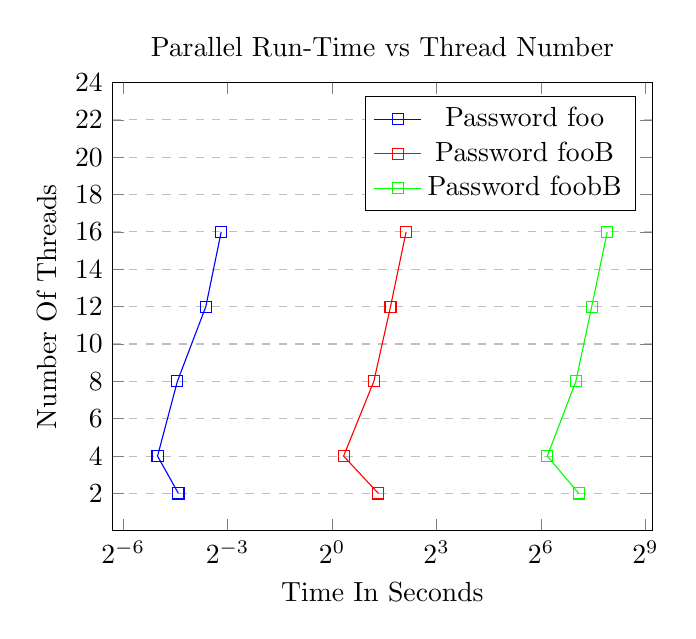
\begin{tikzpicture}
\begin{axis}[
	x tick label style={/pgf/number format/sci},
	log basis x=2,
	xmode=log,
    title={Parallel Run-Time vs Thread Number},
    xlabel={Time In Seconds},
    ylabel={Number Of Threads},
    ymin=0, ymax=24,
    ytick={2,4,...,24},
    legend pos=north east,
    ymajorgrids=true,
    grid style=dashed,
]

\addplot[
    	color=blue,
    	mark=square,
    ]
    coordinates {
    	(4.7e-2,2)(3.1e-2,4)(4.6e-2,8)(8.1e-2,12)(1.1e-1,16)
    };
\addlegendentry{Password foo}
    
\addplot[
    	color=red,
    	mark=square,
    ]
    coordinates {
    	(2.512e0,2)(1.257e0,4)(2.294e0,8)(3.198e0,12)(4.359e0,16)
    };

\addlegendentry{Password fooB}
   	
\addplot[
    color=green,
    mark=square,
    ]
    coordinates {
    (1.35311e2,2)(7.2467e1,4)(1.27841e2,8)(1.7523e2,12)(2.38717e2,16)
    };

\addlegendentry{Password foobB}

\end{axis}
\end{tikzpicture}
\caption{Run-Time vs Number Of Threads Graph}
\end{figure}

As we can see from the above graph, the performance of the parallel version depends from the number of the thread used.\\
In particular since the test were done using a CPU that has two cores and four hardware threads then the optimal number of required 
workers threads is four.\\
In fact, if we use two threads then the application takes a little longer to complete and it can be seen from the Vtune profiler that
the Core usage has dropped:\\
\begin{figure}[H]
\centering
\includegraphics[width=0.5\textwidth]{vtune_profiler_under_usage}
\caption{Intel's VTune-Profiler showing non-optimal thread usage}
\end{figure}
if we increase the number of worker threads then the logical core usage is almost the same but the performance starts to drop due to the 
overhead required to manage the software threads that have to be scheduled by the system:\\
\begin{figure}[H]
\centering
\includegraphics[width=0.5\textwidth]{vtune_profiler_over_usage}
\caption{Intel's VTune-Profiler showing non-optimal thread usage}
\end{figure}

\section{Conclusions}
As we have seen in the metric section the overall performance of the parallel version is two times faster than the sequential version,
and even in simple cases, like the first result, the parallel version is still faster than the sequential one thanks to the usage of 
multiple threads.\\
It is important to note,as seen in section \ref{run-time-vs-num-threads}, that in case of higher core CPU, the program should 
be instructed to use them by specifying the right number of workers threads.\\
\end{document}
